%-*- mode: latex ; mode: visual-line; mode: flyspell ; -*-
\documentclass[12pt,geometry,width=8in]{article}
\usepackage{lastpage}
\usepackage[letterpaper,left=1.5cm,top=1.5cm,right=1.5cm,bottom=2cm]{geometry}
\usepackage[colorlinks=true,urlcolor=blue]{hyperref}
\usepackage{fancyhdr}
\pagestyle{fancy}
\fancyhead{}
\setlength{\parindent}{0pt}
\usepackage[shortlabels]{enumitem}
\usepackage{epigraph}
\renewcommand{\epigraphflush}{center}
\renewcommand{\epigraphwidth}{\textwidth}
\usepackage{verbatim} % to include git info



\usepackage{physics}
\usepackage{graphicx}
\usepackage{enumitem}
\graphicspath{{./figures/}}

\begin{document}
\chead{}
\cfoot{\thepage \space of \pageref*{LastPage}}
\renewcommand{\headrulewidth}{0pt}

\begin{center}
  {\large
    Electricity and Magnetism 3 --- Phys 442  \\
    University of Waterloo, Fall 2020
    --- Problem Set 1\footnote{Thank you to Niloofar Abbasvandi for setting the original problem set and Andrew Kovachik for converting to latex.  The up-to-date latex source code for this problem set is at: \url{https://github.com/jddmartin/phys442_fall2020_problem_set_1}
}
    \par
  }
\end{center}

\vspace{0.1in}

Due Tuesday October 20th, by 17:00EDT.  Submit through Crowdmark.

\vspace{0.1in}

\noindent

\begin{enumerate}[(1),topsep=0pt,itemsep=0ex,partopsep=1ex,parsep=1ex]
\item
\begin{enumerate}[(a)]
\item A parallel plate capacitor is formed of two flat rectangular perfectly conducting sheets of dimensions $a$ and $b$ separated by a distance $d$, which is small compared to $a$ or $b$. Current is fed in and taken out uniformly along adjacent edges of length $b$.  Take current flow to be parallel to the $x$ axis. With time-harmonic input current and voltage defined at this end of the capacitor:

\begin{enumerate}[(i)]
\item Calculate the input impedance or admittance.
\item Calculate the electric and magnetic fields in the capacitor correct to second order in powers of the frequency $\omega$, but neglecting fringing fields.

Hint:

\[
E = E_0 + \omega E_1+ \omega^2 E_2 + \dots
\]

\[
B = B_0 + \omega B_1+ \omega^2 B_2 + \dots
\]

\[
\vb{E}(x) = E(x) e^{-i \omega t}\vu{z}
\]

\[
\vb{B}(x) = B(x) e^{-i \omega t}\vu{y}
\]
\end{enumerate}

Clarification: please note that $\vb{E}$ and $\vb{B}$ depend on the $x$ coordinate (correction from original statement of problem), and that the current flow is parallel to the $x$ axis.

\newpage
\item

\begin{figure}[h]
    \centering
    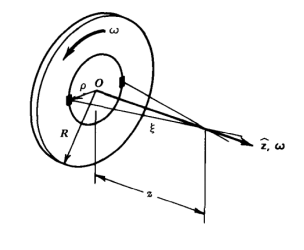
\includegraphics[width=0.5\textwidth]{disk}
    \caption{Diagram for question 1b}
    \label{disk}
\end{figure}

A uniformly charged thin disk of surface charge density $\sigma$, radius $R$, and thickness $t \ll R$ rotates with an angular velocity $w$ about the $z$ axis of symmetry, as shown in figure \ref{disk}.

\begin{enumerate}[(i)]
\item Find the magnetic field at the point located on the $z$ axis of symmetry.
\item Obtain the solution for a sphere of volume charge density $\rho_0$ and the same radius.
\end{enumerate}

Clarification: the disk does not have a hole in the center.

\newpage
\item

\begin{figure}[h]
    \centering
    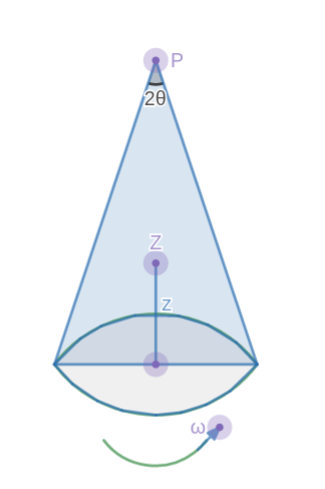
\includegraphics[width=0.3\textwidth]{cone}
    \caption{Diagram for question 1c}
    \label{cone}
\end{figure}

A hollow cone (like a party hat!) has a vertex angle, $2\theta_0$. The radius on the base is $R$ and the height is $H$. It has a surface charge density, $\rho$. It spins around its symmetric axis with angular frequency $\omega$. What is the magnetic field at the top vertex (point P) and the point $Z$ at the distance $z$ from the bottom?
\end{enumerate}

\newpage

\item
\begin{enumerate}[(a)]
\item
\begin{figure}[h]
    \centering
    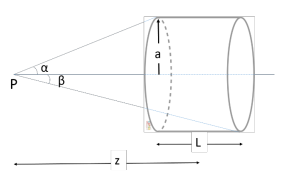
\includegraphics[width=0.5\textwidth]{solenoid}
    \caption{Diagram for question 2a}
    \label{solenoid}
\end{figure}
The magnetic field due to a ring of current of radius $a$, distance $z$ away on the axis of the ring is given by
\[
\frac{\mu_0I}{2a} \sin^3(\theta),
\]
where $\tan\theta = a/z$.  You may use this result in your calculations. Consider a short, (not ideal) solenoid as shown in the figure \ref{solenoid}, of length $L$, number of turns per unit length $n$, radius $a$, and current $I$ flowing through its turns.

\begin{enumerate}[(i)]
\item Find the magnetic field due to the short solenoid, on the axis of the solenoid, on the axis of the solenoid at the point $P$ at a distance $z$ away from the center of the solenoid. $P$ is outside the solenoid. Give the answer in terms of the angles $\alpha$ and $\beta$, where $\alpha$ and $\beta$ are defined in the figure.
\item
Find the magnetic field at the center of the short solenoid when the diameter of the solenoid is equal to its length.
\item
Find the limit of the field at the center of the solenoid when the length of the solenoid is much larger than the diameter. Is this what you expect? Explain.
\item
Does Ampere's law hold for the case of the short solenoid? Explain and elaborate.
\end{enumerate}
\newpage

\item
\begin{enumerate}[(i)]
\item
Show that the energy of the magnetic field of a stationary current distribution $\vec{j}(\vec{x})$ in vacuum is determined by:

\[
W = \frac{\mu_0}{8\pi} \int d^3\vec{x} \int d^3\vec{x}' \: \frac{\vec{j}(\vec{x}) \cdot
\vec{j}(\vec{x}')}{\abs{\vec{x}-\vec{x}'}}
\]

\item
The energy of a system of $n$ current carrying conductors (current $I_i$) can be described by the
quadratic form

\[
W = \frac{1}{2} \sum\limits_{i=1}^n L_i I_i^2 + \sum\limits_{i=1}^n\sum\limits_{j>i}^n L_{ij} I_i
I_j
\]


Find the expression for the self-induction coefficients $L_i$ and the mutual induction coefficients,
$L_{ij}$.

\item
\begin{figure}[h]
    \centering
    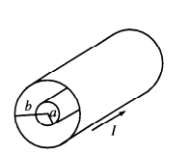
\includegraphics[width=0.25\textwidth]{cyl}
    \caption{Diagram for 2b}
    \label{cyl}
\end{figure}

Calculate the self-induction coefficient in (b) for a long current-carrying coaxial line (as in figure \ref{cyl}). Let the inner conductor (radius $a$) have the permeability, $\mu_0$. The space between the conductors should be filled with a material of permeability, $\mu$.
\end{enumerate}

\item
A solenoid of radius $R$ with $n$ turns per unit length, carries a stationary current, $I$. Two hollow cylinders of length $l$ are fixed coaxially and freely rotation. One cylinder of radius, $a$, is insider the coil ($a<R$) and carries the uniformly distributed charge, $Q$. The other cylinder of radius, $b$ ($b>R$) carries the charge, $-Q$. If the current is switched off the cylinders start to rotate. What is the value of the angular momentum? Where does the angular momentum come from?

Clarification: the charge is only located on the curved surfaces of the cylinders.

\end{enumerate}

\end{enumerate}


\end{document}
